\chapter{Wavetable mit Modifier}


\begin{enumerate}[a)]
% a)
\item

% b)
\item

% c)
\item
Die drei nachfolgenden Grafiken zeigen den Inhalt der Wavetable zu jeweils verschiedenen Zeitpunkten.

\begin{figure}[H]
    \center
    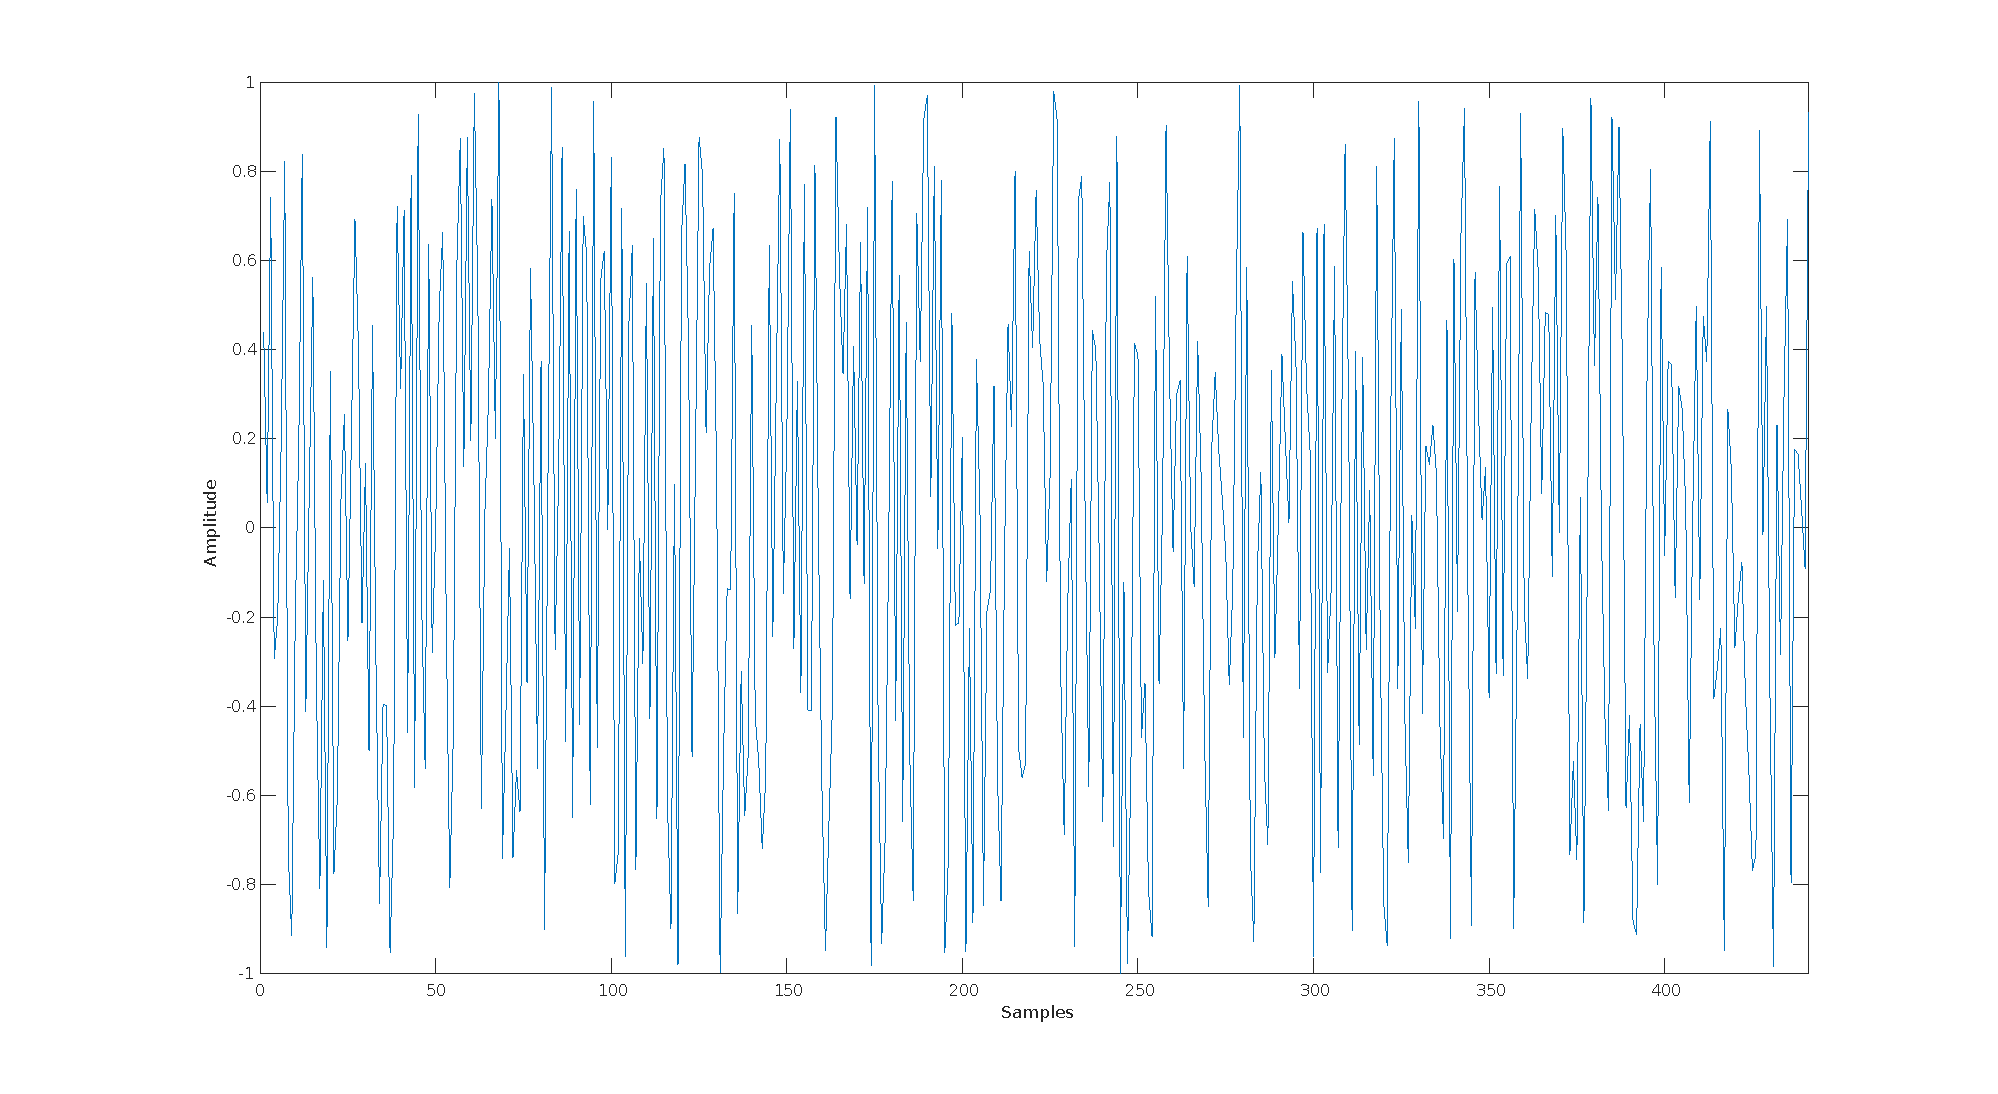
\includegraphics[width = 0.7\textwidth]{Figures/Anfang.pdf}
    \caption{Die Wavetable zu Beginn der Synthese.}
    \label{fig:bs1}
\end{figure}

In dieser Grafik ist die Wavetable in der ersten Iteration des Algorithmus zu sehen.
Das Signal hat einen stark rauschhaften Charakter.
Es lässt sich klar erkennen, dass der Ton aus einem weißen Rauschen generierte wurde. 

\begin{figure}[H]
    \center
    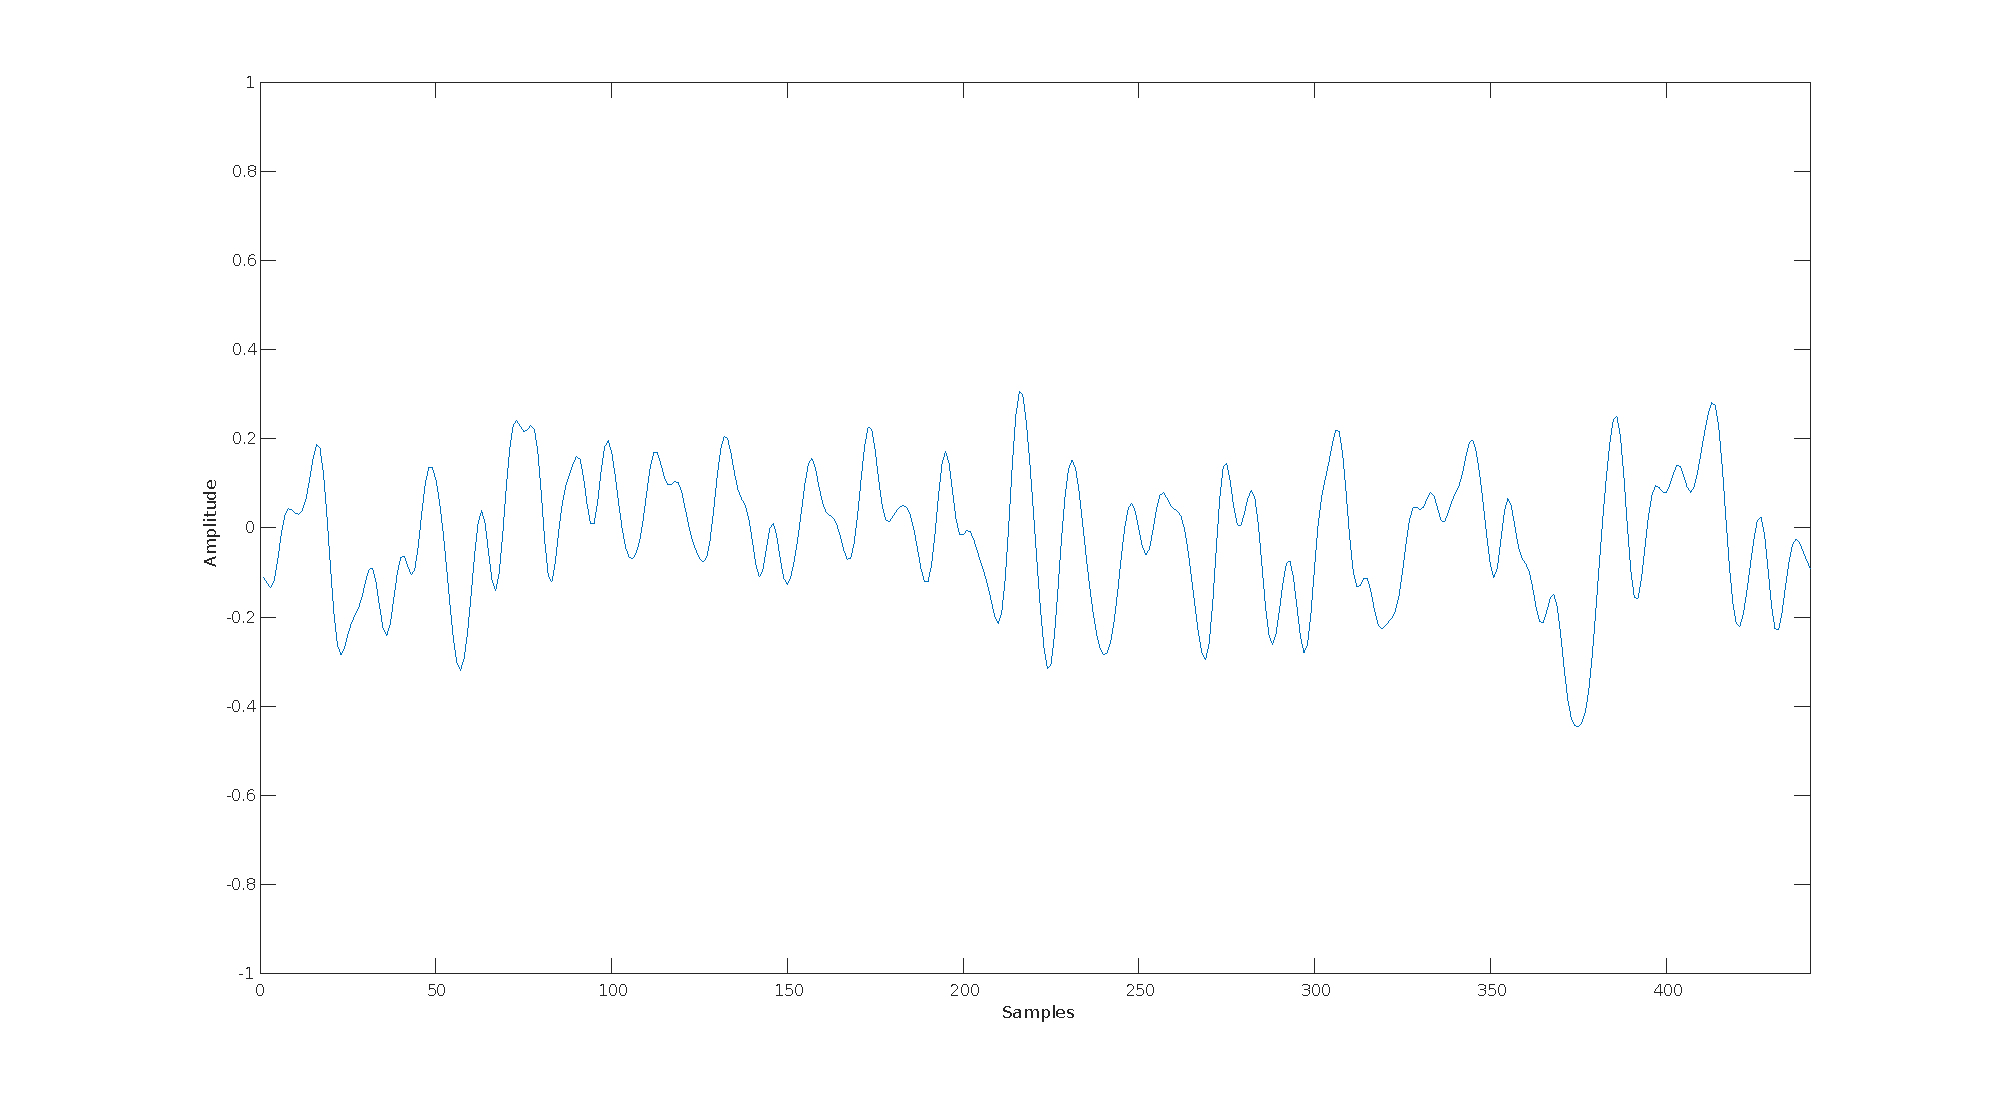
\includegraphics[width = 0.7\textwidth]{Figures/Mitte.pdf}
    \caption{Die Wavetable während der Synthese.}
    \label{fig:bs1}
\end{figure}

Der zweite Plot wurde nach einigen wenigen Iterationen des Algorithmus erstellt.
Hier ist die Glättung, welche durch den gleitenden Mittelwert zu Stande kommt gut zu sehen.
Der rauschhafte Charakter des Signals ist verschwunden.
Die Wellenform erinnert nun eher an eine harmonische Schwingung.
Auch der Effekt des Gains ist bereits stark zu erkennen.
Die ursprüngliche Amplitude wurde bereits stark abgeschwächt.

\begin{figure}[H]
    \center
    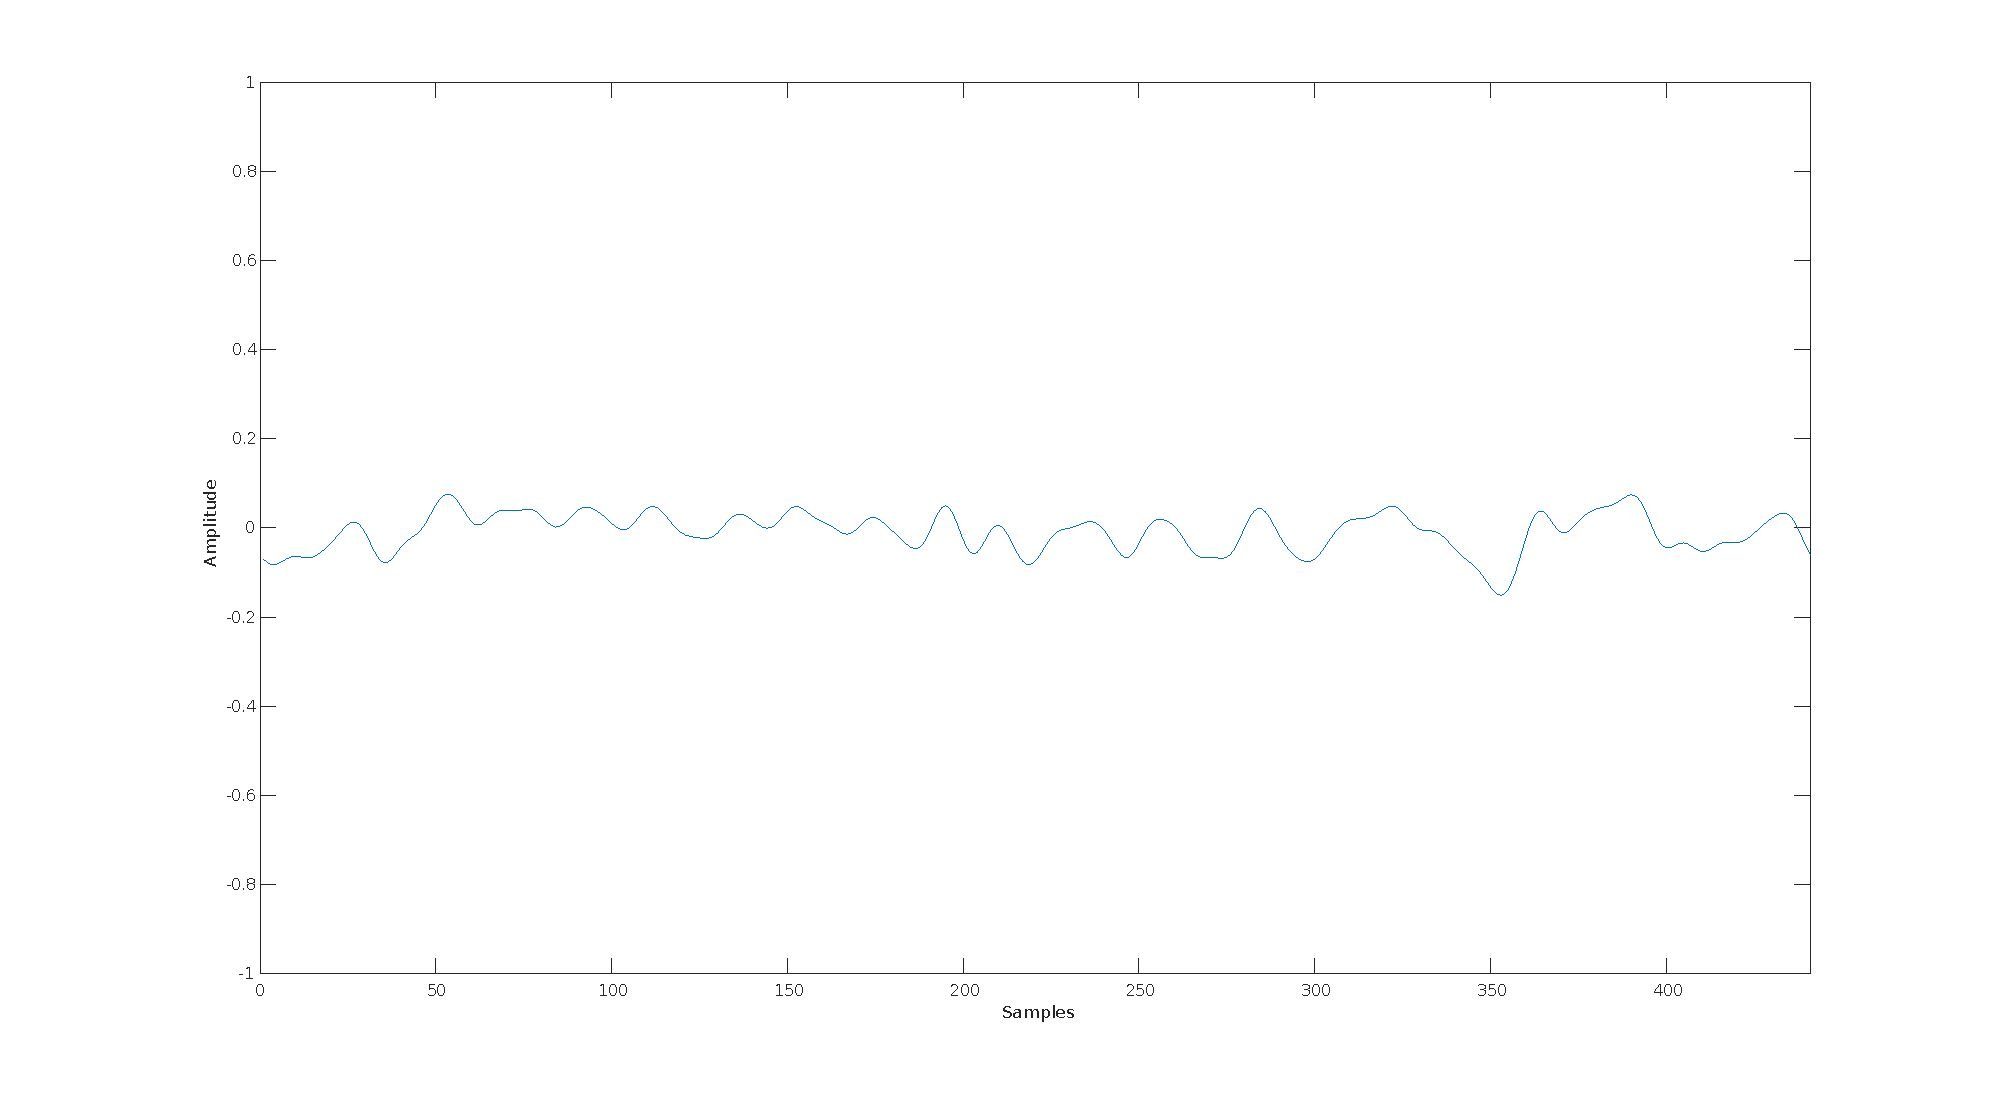
\includegraphics[width = 0.7\textwidth]{Figures/Ende.pdf}
    \caption{Die Wavetable gegen Ende der Synthese.}
    \label{fig:bs1}
\end{figure}

Der letzte Plot ist gegen Ende der 3 Sekunden aufgenommen.
Die Auswirkung des Gains ist hier klar zu erkennen. 
Das Signal ist deutlich abgeschwächt und klingt aus.

% d)
\item

% e)
\item

\end{enumerate}
